\documentclass{article}
\usepackage{graphicx}
\usepackage[left=1in, right=1in, top=1in, bottom=1in]{geometry}
\usepackage{parskip}
\usepackage{amsfonts}
\usepackage{xcolor}
\usepackage{amsmath}
\usepackage{enumitem}
\usepackage{array}

\usepackage{pgfplots}
\pgfplotsset{compat=1.18}

\usepackage{listings}
\lstset{
    language=Python,
    breaklines=true,
    breakatwhitespace=true,
    columns=fullflexible,
    basicstyle=\ttfamily\small,
    numbers=left,
    numberstyle=\tiny\color{gray},
    stepnumber=1,
    numbersep=8pt,
    xleftmargin=2em,
    framexleftmargin=2em,
}

% \usepackage{minted}

\graphicspath{ {./images/} }

\title{GPU Option Pricing Project Notes}
\author{Ethan Kim}
% \date{2026/03/27}

\begin{document}
\maketitle
\section*{Introduction}
This is my first quantitative finance project.
The project is a ``Monte Carlo engine for pricing path-depending exotic options''.
As a beginner in the space, Gemini was used to create, plan, and help walk through the project. 

This project is broken down into three stages
\begin{enumerate}
    \item Stage 1: Python/NumPy Baseline
    
    In this stage, I learn the formulas that I will later have to implement in code like the GBM formula and the pricing methods for Asian and Down-and-Out Barrier call options.
    I also implement these functions using NumPy (since NumPy has convenient functions). 
    \item Stage 2: C++ Rewrite with SIMD Optimization
    
    In this stage we translate our Python code into C++ code and add some basic optimizations.
    Some of these optimizations include, using a single ``flat'' array, avoiding unecessary calculations, and AVX2 (an instruction set expansion that uses larger registers)
    \item Stage 3: CUDA GPU Implementation
    
    In this stage, we take our calculations to the GPU by taking advantage of NVIDIA T4 GPUs (provided for free in Colab) and writing programs in CUDA (programming model that allows programmers to ``talk'' with NVIDIA GPUs)
\end{enumerate}

\newpage
\section*{Stage 1: Python/NumPy Baseline}
In this section, we are going to write python programs using NumPy to generate GBM paths and price asian and barrier option calls.
This is simply as a practice (since I am more familiar with Python)
\subsection*{Log-Normal vs Normal Distribution}
Typically in quantitative finance, we model the price of an asset using the Log-Normal distribution rather than the Normal.

As a reminder, for a random variable \(X\) to be log-normal distributed, this means that \(\ln(X)\) should be normally distributed. 

\begin{figure}[htbp] % [h]ere, [t]op, [b]ottom, [p]age
    \centering
    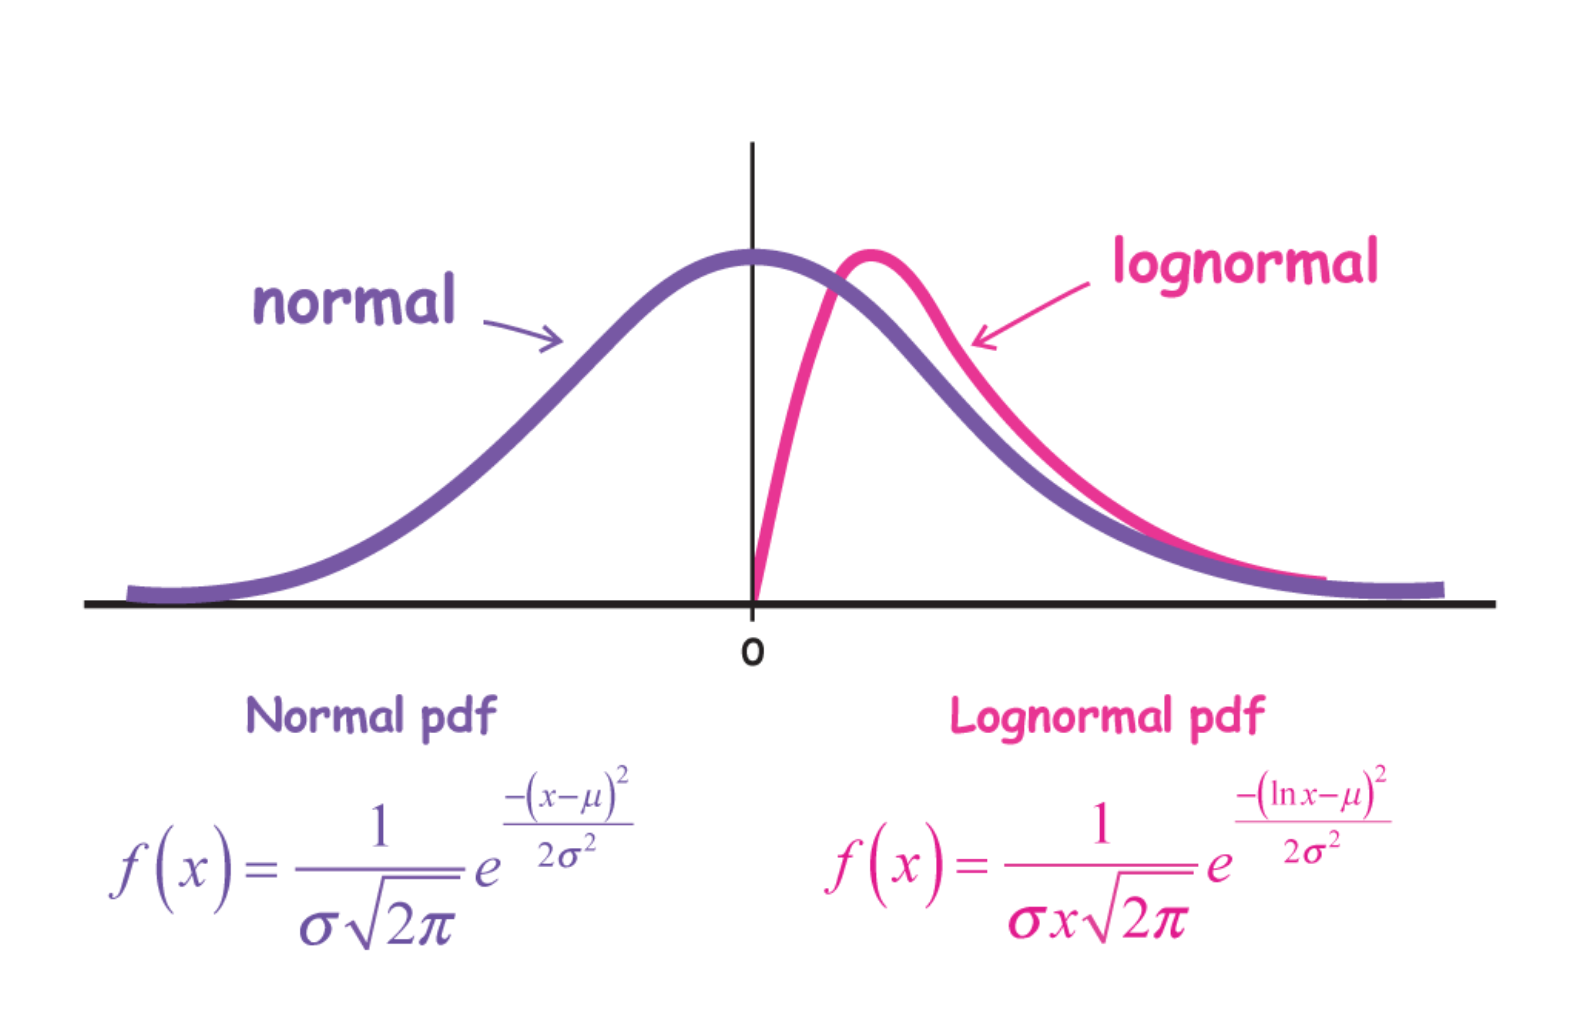
\includegraphics[width=0.5\textwidth]{lognormalvsnormal.png}
    \caption{Normal vs Lognormal}
    \label{fig:label_name}
\end{figure}

As we can see, the lognormal distribution has two important features that make it a better candidate for modeling asset prices.

The first is that the log normal does not go below zero.
Since we are modeling the price of an asset itself, and not the gain or loss, the value of the random variable should never go below zero.

Another feature of the lognormal distribution that is important is its right skew.
Think about the price of an asset, theoretically it could rise by any amount, but it can only fall by its total value.
Overtime, a series of good returns can compound dramatically while losses are bounded by zero.

\subsection*{Geometric Brownian Motion (GBM)}
When we simulate asset price, we need to define a rule for how the price moves from time \(t\) to time \(t+\,dt\).
If we don't define this rule, we are just simulating random noise. 

Typically in quant finance, we use Geometric Brownian Motion because it has two essential features
\begin{enumerate}
    \item Drift \((\mu)\): This is the average rate of return you expect the asset to return.
    \item Volatility \((\sigma)\): This is the random "noise" or risk
\end{enumerate}

\begin{figure}[htbp] % [h]ere, [t]op, [b]ottom, [p]age
    \centering
    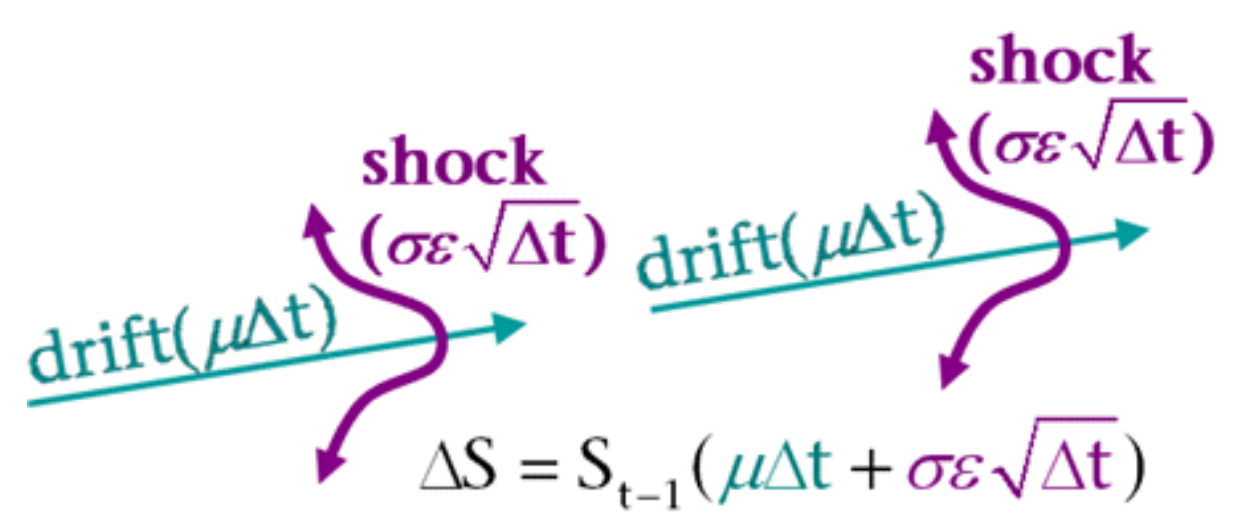
\includegraphics[width=0.5\textwidth]{driftvolatility.png}
    \caption{Visualizing Drift and Volatility}
    \label{fig:label_name}
\end{figure}

If the volatility was just zero \((\sigma=0)\), then the price would just grow smoothly at rate \(\mu\) like a savings account

A stochastic process \(S_t\) is said to follow GBM if it satisfies the following stochastic differential equation
\[dS_t=\mu S_t\,dt+\sigma S_t \,dW_t\]

For some arbitrary initial \(S_0\), the SDE has the following solution
\[S_t=S_0\exp\left(\left(\mu-\frac{\sigma^2}{2}\right)t+\sigma W_t\right)\]

Notice how in the analytical solution we are subtracting \(\frac{\sigma^2}{2}\) from \(\mu\).
The reason why we do this is because there is a difference between the average return and the actual result which is known as volatility drag.
Volatility is symmetric in log-return space, but asymmetric in price space. 
Consider a 10\% increase in price followed by a 10\% decrease. You don't return to where you started. 

\subsection*{Vectorized Path Generation in NumPy}
To get a statistically significant price for an asset, it does not suffice to model 1, 10, or even 100 paths.
We might need 100,000 or even 1,000,000. 

A naiive approach would be to use a simple for loop to simulate each of the paths, but this would be very slow.
Instead, we will take advantage of vectorization to perform operations on entire arrays at once (this mirrors how the GPU will eventually work).

We are now going to define a function \texttt{generate\_gbm\_paths} which will generate all of our paths.

The parameters of this function are \texttt{S0} (initial price), \texttt{mu} (drift), \texttt{sigma} (volatility), \texttt{T} (time to maturity in years), \texttt{steps} (number of time increments), \texttt{paths} (number of simulations)

The output of this function should be a NumPy array of shape \texttt{(steps+1,paths)} (each column of this array will represent a single path)

As a reminder, the discrete version of the GBM formula is \[S_{t+\Delta t}=S_t\exp\left(\left(\mu-\frac{\sigma^2}{2}\right)\Delta t+\sigma\sqrt{\Delta t}Z\right)\]

Using this formula, if we know \(S_0\), there is a simple expression to find \(S_t\) rather than taking \(t\) discrete update steps (which would be a computational nightmare for high number of \texttt{steps} and \texttt{paths})

Let's look at the pattern (ket \(X_t\) be the inner portion of the \(\exp\))
\[S_1=S_0\exp(X_1)\]
\[S_2=S_1\exp(X_2)=S_0\exp(X_1)\exp(X_2)\]

The general formula is \[S_t=S_0\exp(\sum_{i=1}^{t}X_i)\]

\subsubsection*{Python Code generate\_gbm\_paths}

\begin{lstlisting}
    def generate_gbm_paths(S0, mu, sigma, T, steps, paths):
        delta_t = T / steps
        standard_normal_samples = np.random.standard_normal(size=(paths, steps))
        volatility_drag = (mu - (sigma ** 2) / 2) * delta_t
        inner_exp = standard_normal_samples * (sigma * np.sqrt(delta_t)) + volatility_drag
        summed = np.cumsum(inner_exp, axis=1)
        zero_start = np.concatenate((np.zeros((paths, 1)), summed), axis=1)
        paths = np.exp(zero_start) * S0
        return paths
\end{lstlisting}

Line 4 creates an array of samples of the standard normal. These are the \(Z\)'s for each step of each path

Line 6 sums up the volatility drag and the scaled normal samples

Line 8 sums up the \(X_i\)'s. So at this point index \([x,y]\) represents \(X_x\) for path \(y\)

Line 9 puts an array of \(S_0\)'s at the beginning to simulate time 0

Lines 10 and 11 apply the \(\exp\) and multiply by \(S_0\)

\subsection*{Asian Option Payoff}
Unlike American and European options which depend on the asset's price at a specific point, an Asian option pays iooff based on the average price of the asset over time.

Some reasons why one would want to use Asian options are 
\begin{enumerate}
    \item Manipulation resistance: averaging the value of an option over many days makes it harder for someone to try to pin (when large firms artifically push the price up or down by placing massive orders) or manipulate the price on expiry day
    \item Cheaper/better matches real exposures: averaging smooths out volatility. For a company that justs wants to hedge a steady exposure (many coporate gedging needs are inherently about average prices over a period), paying for a full European option's volalility is wastful
\end{enumerate}

Asian options generally don't have simple closed for solutions
(the average of log-normally distributed variables is itself not log-normal).
This is why GBM simulation is particularly useful.
You simulate many fulls paths, compute the average price along each path, calculate the payoff, and discount the expected payoff back.

The payoff for a standard ``fixed-strike'' Asian call option is defined as \[C(T)=\max(A(0,T)-K,0)\] where \(A\) denotes the average price for the period \([0,T]\) and \(K\) is the strike price.

(Note that when an article says \([0,T]\), it typically inplies a continuous integral \(A=\frac{1}{T}\int_{0}^{T}S_t\,dt\).
In the dicrete case, since Day 0 is already known, it is often excluded because it isn't ``risky'')

We will now write a python function \texttt{price\_asian\_call} that will calculate the fair price today of the Asian call option.

We do this by taking the average price of the asset,
subtract the strike price,
take the \(\max\) of those values with zero (your losses can never go below zero),
subtracting the discount (the value of the dollar in the future might be different than it is today \(e^{-rT}\)),
and finally average this value across all the paths to get the average.

\subsubsection*{Python Code price\_asian\_call}
\begin{lstlisting}
    def price_asian_call(paths, K, r, T):
        mean = np.mean(paths[:, 1:], axis=1)
        sub_strike = mean - K
        call_rule = np.maximum(sub_strike, 0)
        avg = np.mean(call_rule)
        discount = avg * np.exp(-r * T)
        return discount
\end{lstlisting}

Line 2 slices out the day 0 data from the array

In line 5 and 6, rather than multiplying by the discount and then taking the average, we take the average first which saves thousands of compuations

\subsection*{The Barrier Option}
Barrier options are another type of exotic option.
Unlike the Asian option where the path determines the amount of the payoff,
a barrier option uses the path to determine if the option exists at all.

\begin{enumerate}
    \item Knock-in: type of barrier option where the rights associated with the option only come into existence when the price of the asset reaches a specified barrier during the option's life
    \begin{enumerate}
        \item up-and-in: option only comes into existence if the price of the asset rises above the pre-specified barrier (set above initial price)
        \item down-and-in: option only comes into existence if the price of the asset falls below the pre-specified barrier (set below initial price)
    \end{enumerate}
    \item Knock-out: this option ceases to exist if the underlying asset reaches a barrier
    \begin{enumerate}
        \item up-and-out: ceases to exist if the price rises above a the barrier (set above initial price)
        \item down-and-out: ceases to exist if the price falls below a barrier (set below inital price)
    \end{enumerate}
\end{enumerate}

So now instead of just calculating averages, we are looking for a breach across the barrier.

For a down-and-out call, the payoff at \(T\) is \[\text{Payoff}=\max(S_T-K,0)\cdot1_{\{\min(S_t)>B\}}\]

We will now write a function called \texttt{price\_barrier\_out\_call}. This function returns the fair price today of a down-and-out barrier call option.

We do this by going through each of the paths and checking to see if at any time step the price fell below the barrier.

\subsubsection*{Python Code price\_barrier\_out\_call}
\begin{lstlisting}
    def price_barrier_out_call(paths, K, B, r, T):
        terminal_prices = paths[:, -1]
        payoffs = np.maximum(terminal_prices - K, 0)
        mask = ~np.any(paths < B, axis=1)
        survived = payoffs * mask
        avg = np.mean(survived)
        discount = avg * np.exp(-r * T)
        return discount
\end{lstlisting}

Notice how in line 4 there's a \(\sim\). Thios is because \texttt{np.any(paths<B,axis=0)} will return \texttt{True} if the price hit the barrier. 
However, we want to exclude these paths, so we have to do a bitwise NOT operator to turn \texttt{True} into \texttt{False} and vice versa.

\subsection*{Validation}
Monte Carlo Simulation is just a numerical approximation.
The purpose of this validation is to ensure that our approximation converges to the actual truth.
I was wondering why we are doing MC simulations when we already have closed-form solutions,
and this is because closed-form solutions have a lot of assumptions (for example that the world follows GBM which has constant volatiliy).
If we move to a different model like the Heston Model which treats volatility as a random process, the closed-form solutions that we have breaks.

For this step we are going to generate paths, determine the prices for the Asian and Barrier options, and then compare it to the price that the analytical formula gives us.

Note that for the Asian call, since we used the arithmetic average instead of the geometric average, there is no closed-form solution.
To test the validity of our Asian call price function, we check stability by running the simulation multiple times and checking that price doesn't jump around wildly.

Using these (\texttt{S0=100, K=100, B=90, r=0.05, sigma=0.2, T=1.0}) parameters for the barrier call analytical price, we get a price of 8.6655.
Running the MC simulation with the same parameters and \texttt{steps=1000, paths=100000}, we get a price of 8.8408.
The MC simulation is \(\sim17\) cents off. This difference can be attributed to the analytical formula assuming continuous monitoring, while the simulation uses 1000 discrete time steps.
Increasing the steps to 5000 results in a simulated price of 8.7459 which is an improvement over 1000 steps. 

Running the simulation five times with the same GBM parameters on different seeds resulted in these prices \([5.7232,5.7434,5.7601,5.7468,5.7326]\).
This is a good sign, it shows that the simulation is stable and consistent.

\section*{Stage 2: C++ Rewrite with SIMD Optimization}
In this stage, we are going to translate our Python code to C++ and add some optimizations. 
\subsection*{Memory Allocation and ``The Flat Array'' (C++ Rewrite)}
In Python, when we create a 2D array like \texttt{np.random.standard\_normal(size=(steps, paths))} Python creates a sophisticated object that manages that data for us.
However, the overhead associated with such a storage method is disasterous for HFT. 

In high performance C++, we tend to avoid ``array of arrays'' (vectors in C++).
Instead we use a flat array.
This is because CPUs are able to work faster when they can read memory in a stright line.
Remember spacial locality: the tendency of a computer program to access memory locations close to recently accessed data within a short time frame.

So instead of a 2D array with dimensions \texttt{steps*paths}, we make a single long \texttt{paths*steps} array 
(it's actually \texttt{paths*(steps+1)} because of the step 0).

Since we are using a single dimention vector to store 2D data, we need a way to convert 2D coordinates into 1D indicies.
The formula that you use depends on whether you are storing the store the data in row-major or column-major order.
In this project, we are storing the data in row-major order which means that elements in a row are stored in contiguous memory locations.

The formula for calculating the array index \((i)\) of a 2D array coordinate \((r,c)\) using row-major order is this \[i=r\cdot\text{width of array}+c\]

\subsubsection*{C++ Code generate\_gbm\_paths}
\begin{lstlisting}[language=C++]
    std::vector<double> generate_gbm_paths(double S0, double mu, double sigma, int T, int steps, int paths, std::mt19937& gen) {
        std::normal_distribution<double> d(0.0, 1.0);
        std::vector<double> paths_matrix(paths * (steps + 1), 0.0);
        double delta_t = static_cast<double>(T) / steps;
        double volatility_drag = (mu - (sigma * sigma) / 2.0) * delta_t;
        double normal_scalar = sigma * std::sqrt(delta_t);

        for (int i = 0; i < paths; i++) {
            paths_matrix[i * (steps + 1)] = S0;
        }

        for (int i = 0; i < paths; i++) {
            for (int j = 1; j <= steps; j++) {
                double random = d(gen);
                int cur_index  = i * (steps + 1) + j;
                int prev_index = i * (steps + 1) + (j - 1);
                paths_matrix[cur_index] = paths_matrix[prev_index] * std::exp(volatility_drag + normal_scalar * random);
            }
        }
        return paths_matrix;
    }
\end{lstlisting}

Notice how for constants that are not dependent on the current loop index, we calculate them outside of the for loop to avoid redundant computation.
Some examples of this are the \texttt{delta\_t}, \texttt{volatility\_drag}, and \texttt{normal\_scalar} variables.

Also another computation saving method is creating a larger vector to hold time zero prices instead of appending on a vector at the beginning.
This is because appending a vector requires a shift of every other element.
This that appending time zero prices results in \texttt{path} insertions that each cost \(O(N)\) time.
Pre-allocation is also generally the better practice in performance-sensitive code because you want to avoid unexpected memory movement.

\subsubsection*{C++ Code price\_asian\_call}
\begin{lstlisting}[language=C++]
    double price_asian_call(const std::vector<double>& paths_matrix, double K, double r, double T, int steps, int num_paths) {
        double total_payoff = 0.0;
        for (int i = 0; i < num_paths; i++) {
            auto start = paths_matrix.begin() + i * (steps + 1) + 1;
            auto end   = paths_matrix.begin() + i * (steps + 1) + steps + 1;
            double total   = std::accumulate(start, end, 0.0);
            double average = total / steps;
            double payoff  = std::max(average - K, 0.0);
            total_payoff  += payoff;
        }
        return (total_payoff / num_paths) * std::exp(-r * T);
    }
\end{lstlisting}

Since we stored our paths data in row-major order, we can easily accumulate the prices of a single path to find the average.

\subsubsection*{C++ Code price\_barrier\_out\_call}
\begin{lstlisting}
    double price_barrier_out_call(const std::vector<double>& paths_matrix, double K, double B, double r, double T, int steps, int num_paths) {
        double total_payoff = 0.0;
        for (int i=0; i<num_paths; i++) {
            auto start = paths_matrix.begin() + i * (steps + 1);
            auto end = paths_matrix.begin() + i * (steps + 1) + steps + 1;

            bool broke = std::any_of(start, end, [&B](double price){return price < B;});
            if(!broke) {
                total_payoff += paths_matrix[i * (steps + 1) + steps] - K;
            }
        }
        return (total_payoff / num_paths) * std::exp(-r * T);
    }
\end{lstlisting}

Now that we have both Python and C++ implementations of these functions, we will test them to compare their speeds.
I ran both versions using these parameters (\texttt{S0=100, K=100, B=90, r=0.05, sigma=0.2, T=1.0, steps=252, paths=1000000}).
Here were the results.
\begin{figure}[h]
\centering
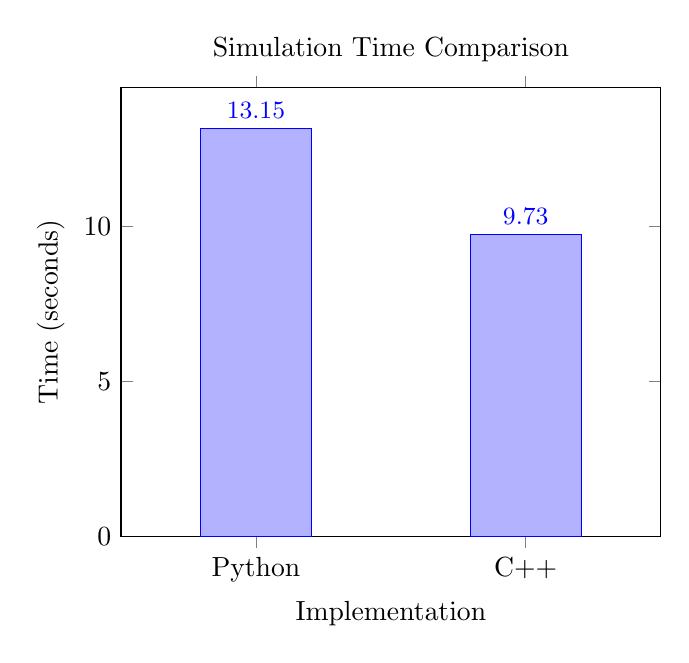
\begin{tikzpicture}
\begin{axis}[
    ybar,
    bar width=40pt,
    ymin=0,
    ylabel={Time (seconds)},
    symbolic x coords={Python, C++},
    xtick=data,
    nodes near coords,
    enlarge x limits=0.5,
    title={Simulation Time Comparison},
    xlabel={Implementation},
    nodes near coords style={font=\small},
]
\addplot coordinates {(Python, 13.1546) (C++, 9.7335)};
\end{axis}
\end{tikzpicture}
\end{figure}

Using C++ and some optimizations to how we store and handle data resulted in a \(\sim1.36\)x speedup.
The main reason for this is due to NumPy's overhead.
NumPy operations like \texttt{np.cumsum, np.exp, np.random.standard\_normal} are separate calls that allocates new arrays.
So while working on the single \texttt{paths} array, numerous sub-arrays are being created and deleted.

However, apparently this performance speedup isn't even that great.
NumPy already uses vectorized instructions, so our optimized C++ code is trying to beat already optimized C++ code with a python wrapper.

What really will takes our code to the next level is explicit SIMD instructions.
Currently we compile our C++ code with the \texttt{-O3 -march=native} flags and hope that the compiler can automatically vectorize operations.
While it often does for simple loops, it fails for more complicated loops like the GBM path generating function.
In this next step, we are giong to call SIMD instructions directly using compiler built-in functions.

\subsection*{SIMD Optimization with AVX2}
AVX2 are SIMD extensions that allows the CPU to perform the same methematical operation on multiple data points simultaneously using wide registers.
For example, if we use floats for the price paths, a single AVX2 register can hold \(\frac{256}{32}=8\) of these values.

\subsubsection*{C++ AVX Optimized Code generate\_gbm\_paths}
% \begin{minted}{cpp}
%     #include "avx_mathfun.h"
%     typedef __m256 v8sf;

%     void generate_gbm_paths_avx_float(float S0, float mu, float sigma, float T, int steps, 
%     int paths, float* data, const float* rng_block)
%     {
%         int num_paths_aligned = (paths + 7) & ~7;

%         float delta_t        = T / static_cast<float>(steps);
%         float volatility_drag = (mu - 0.5f * sigma * sigma) * delta_t;
%         float normal_scalar  = sigma * std::sqrt(delta_t);

%         v8sf v_vol_drag   = _mm256_set1_ps(volatility_drag);
%         v8sf v_norm_scale = _mm256_set1_ps(normal_scalar);
%         v8sf v_s0         = _mm256_set1_ps(S0);

%         for (int i = 0; i < num_paths_aligned; i += 8) {
%             _mm256_store_ps(&data[0 * num_paths_aligned + i], v_s0);
%         }

%         for (int j = 1; j <= steps; j++) {
%             for (int i = 0; i < num_paths_aligned; i += 8) {
%                 v8sf v_rand = _mm256_load_ps(&rng_block[(j - 1) * num_paths_aligned + i]);
%                 v8sf v_prev_price = _mm256_load_ps(&data[(j - 1) * num_paths_aligned + i]);
%                 v8sf v_exponent = _mm256_fmadd_ps(v_norm_scale, v_rand, v_vol_drag);
%                 v8sf v_next_price = _mm256_mul_ps(v_prev_price, exp256_ps(v_exponent));
%                 _mm256_store_ps(&data[j * num_paths_aligned + i], v_next_price);
%             }
%         }
%     }
% \end{minted}
\begin{lstlisting}[language=C++]
    #include "avx_mathfun.h"
    typedef __m256 v8sf;

    void generate_gbm_paths_avx_float(float S0, float mu, float sigma, float T,
                                    int steps, int paths,
                                    float* data, const float* rng_block)
    {
        int num_paths_aligned = (paths + 7) & ~7;

        float delta_t        = T / static_cast<float>(steps);
        float volatility_drag = (mu - 0.5f * sigma * sigma) * delta_t;
        float normal_scalar  = sigma * std::sqrt(delta_t);

        v8sf v_vol_drag   = _mm256_set1_ps(volatility_drag);
        v8sf v_norm_scale = _mm256_set1_ps(normal_scalar);
        v8sf v_s0         = _mm256_set1_ps(S0);

        for (int i = 0; i < num_paths_aligned; i += 8) {
            _mm256_store_ps(&data[0 * num_paths_aligned + i], v_s0);
        }

        for (int j = 1; j <= steps; j++) {
            for (int i = 0; i < num_paths_aligned; i += 8) {
                v8sf v_rand = _mm256_load_ps(&rng_block[(j - 1) * num_paths_aligned + i]);
                v8sf v_prev_price = _mm256_load_ps(&data[(j - 1) * num_paths_aligned + i]);
                v8sf v_exponent = _mm256_fmadd_ps(v_norm_scale, v_rand, v_vol_drag);
                v8sf v_next_price = _mm256_mul_ps(v_prev_price, exp256_ps(v_exponent));
                _mm256_store_ps(&data[j * num_paths_aligned + i], v_next_price);
            }
        }
    }
\end{lstlisting}

(Notice how we moved the RNG out of the function, we still have to generate random numbers, but it is then fed into the function rather than happening inside.
This is advantageous because it allows for flexibility if we want to use different RNG methods, and it's also good for testing and caching.)

(The avx\_mathfun header provides vectorized implementations of functions like \texttt{exp} using methods like taylor series expansion.)

When I run this code on 100,000 paths, I get that the total simulation time takes \(\sim488\)ms with about \(\sim418\)ms used for RNG generation and the other \(\sim69\)ms used for the actual simuation calcuations.

Here are some of the reasons for this speed
\begin{enumerate}
    \item Registers: even though NumPy uses vectorized operations, it creats a lot of temporary arrays that have to be written and read from memory.
    If you have a lot of paths, this results in many reads and writes from memory which is low.
    AVX on the otherhand does all the computations within registers, which the CPU can very quickly write to and read from, before storing the final result in memory.
    \item 8-way Parallelism: since we are using floats (lower precision) in this implementation,  one instruction can now do the work of 8.
    Also operations like \texttt{\_mm256\_fmadd\_ps} can calculate \(a\times b+c\) in the same time it takes to do just the multiplication
\end{enumerate}

\subsubsection*{C++ AVX Optimized Code price\_asian\_call\_avx}
\begin{lstlisting}[language=C++]
    double price_asian_call_avx(const float* data, float K, float r, float T, int steps, int paths) {
        int num_paths_aligned = (paths + 7) & ~7;
        
        v8sf v_K = _mm256_set1_ps(K);
        v8sf v_steps = _mm256_set1_ps(static_cast<float>(steps));
        v8sf v_zero = _mm256_setzero_ps();

        double total_payoff = 0.0;

        for (int i = 0; i < num_paths_aligned; i += 8) {
            v8sf v_sum = _mm256_setzero_ps();
            
            for (int j = 1; j <= steps; j++) {
                v8sf v_price = _mm256_load_ps(&data[j * num_paths_aligned + i]);
                v_sum = _mm256_add_ps(v_sum, v_price);
            }

            v8sf v_avg = _mm256_div_ps(v_sum, v_steps);
            v8sf v_payoff = _mm256_max_ps(_mm256_sub_ps(v_avg, v_K), v_zero);

            alignas(32) float payoffs[8];
            _mm256_store_ps(payoffs, v_payoff);

            int valid_lanes = std::min(8, paths - i);
            for (int k = 0; k < valid_lanes; k++) {
                total_payoff += payoffs[k];
            }
        }

        return (total_payoff / paths) * std::exp(-r * T);
    }
\end{lstlisting}

\subsubsection*{C++ AVX Optimized Code price\_barrier\_out\_call\_avx}
\begin{lstlisting}
    double price_barrier_out_call_avx(const float* data, float K, float B, float r, float T, int steps, int paths) {
        int num_paths_aligned = (paths + 7) & ~7;
        
        v8sf v_K = _mm256_set1_ps(K);
        v8sf v_B = _mm256_set1_ps(B);
        v8sf v_zero = _mm256_setzero_ps();

        double total_payoff = 0.0;

        for (int i = 0; i < num_paths_aligned; i += 8) {
            v8sf v_valid = _mm256_cmp_ps(v_zero, v_zero, _CMP_EQ_OQ);

            for (int j = 0; j <= steps; j++) {
                v8sf v_price = _mm256_load_ps(&data[j * num_paths_aligned + i]);
                v8sf v_cmp = _mm256_cmp_ps(v_price, v_B, _CMP_GE_OQ);
                v_valid = _mm256_and_ps(v_valid, v_cmp);
            }

            v8sf v_final_price = _mm256_load_ps(&data[steps * num_paths_aligned + i]);
            v8sf v_payoff = _mm256_max_ps(_mm256_sub_ps(v_final_price, v_K), v_zero);

            v_payoff = _mm256_and_ps(v_payoff, v_valid);

            alignas(32) float payoffs[8];
            _mm256_store_ps(payoffs, v_payoff);

            int valid_lanes = std::min(8, paths - i);
            for (int k = 0; k < valid_lanes; k++) {
                total_payoff += payoffs[k];
            }
        }

        return (total_payoff / paths) * std::exp(-r * T);
    }
\end{lstlisting}

Here are the benchmark results for 1,000,000 paths (using the same parameters from before)
\begin{center}
    \begin{tabular}{|c|c|}
        \hline
        \multicolumn{2}{|c|}{Results} \\
        \hline
        RNG fill time & 3971.9736 ms \\
        \hline
        GBM simulation time & 867.0618 ms\\
        \hline
        Asian pricing time & 92.6260 ms \\
        \hline
        Barrier pricing time & 224.1603 ms \\
        \hline
        Total execution time & 5255.8217 ms \\
        \hline
    \end{tabular}
\end{center}

Now let's compare the total execution time for the Python, C++, and AVX-Optimized C++ implementations

\begin{figure}[h]
\centering
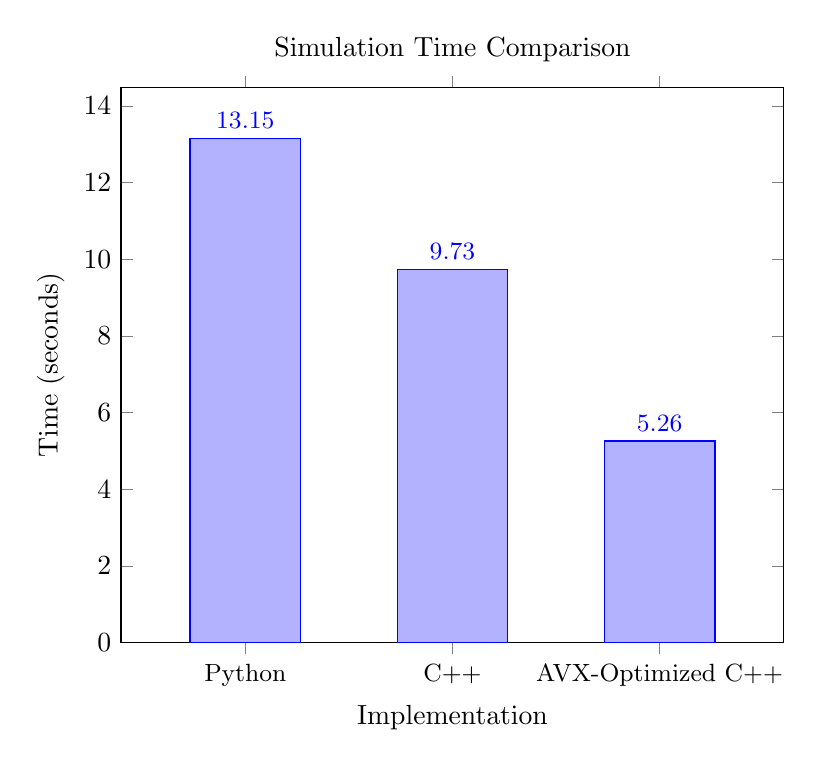
\begin{tikzpicture}
\begin{axis}[
    ybar,
    width=10cm,
    bar width=40pt,
    ymin=0,
    ylabel={Time (seconds)},
    symbolic x coords={Python, C++, AVX-Optimized C++},
    xtick=data,
    nodes near coords,
    enlarge x limits=0.3,
    title={Simulation Time Comparison},
    xlabel={Implementation},
    nodes near coords style={font=\small},
    x tick label style={font=\small}, % slightly smaller labels
]
\addplot coordinates {(Python, 13.1546) (C++, 9.7335) (AVX-Optimized C++, 5.2558)};
\end{axis}
\end{tikzpicture}
\end{figure}

\section*{Stage 3: CUDA GPU Implementation}
While the speedups we saw using AVX-optimized SIMD instruction were impressive, all this work in still happening on the CPU.
There is still room for improvement.
A lot of the calculations that we are doing in this simulation is non-sequential, meaning that we don't have to wait for some previous thing to finish before continuing. 
For example, each path independent, so we can have hundreds of threads, each thread working through a single path. 

In AVX, you manually manage the different lanes in a register.
In CUDA on the other hand, you write code for a single thread, and it executes that thread across a ``warp'' (32 threads)

To practice bridging the gap between the CPU (host) and the GPU (device), we are going to write a small program that allocates memory on the host and device, does work on the device, and moves it back to the host.

\subsubsection*{CUDA Code Simple Program}
\begin{lstlisting}[language=C++]
    // Kernel that sets every element to a given value
    __global__ void initS0(float* devA, float value) {
        int idx = threadIdx.x + blockIdx.x * blockDim.x;
        devA[idx] = value;
    }

    int main() {
        const int paths = 1024;

        // 1. Allocate host array and initialize to 0.0f
        float* A = nullptr;
        cudaMallocHost(&A, paths * sizeof(float));
        for (int i = 0; i < paths; i++) A[i] = 0.0f;

        // 2. Allocate device array
        float* devA = nullptr;
        cudaMalloc(&devA, paths * sizeof(float));

        // 3. Launch kernel: 1 block, 1024 threads
        initS0<<<1, paths>>>(devA, 100.0f);
        cudaDeviceSynchronize();

        // 4. Copy results back to host
        cudaMemcpy(A, devA, paths * sizeof(float), cudaMemcpyDeviceToHost);

        // 5. Print first 5 values to verify
        printf("First 5 values:\n");
        for (int i = 0; i < 5; i++) {
            printf("A[%d] = %.2f\n", i, A[i]);
        }

        cudaFree(devA);
        cudaFreeHost(A);
        return 0;
    }
\end{lstlisting}
In the kernel, each of the 1024 threads gets a unique \texttt{idx} and writes \texttt{100.0f} to its own slot in the array, all simultaneously

\texttt{cudaMallocHost} allocates memory on the host.
Using this allocates a ``page-locked'' host array which is faster for GPU transfers that normal \texttt{malloc}

\texttt{cudaMalloc} allocates memory on the GPU

\texttt{initS0<<<1, paths>>>} launches a kernel with 1 block of 1024 threads. 
CUDA organizes threads using a two-level hierarchy.
First the entire launch is broken down into blocks, and then each block is broken down into threads.
This is just one of the configurations that we could have done, we could have instead launched \texttt{<<<4, 256>>>}

\texttt{cudaDeviceSynchronize} forces the CPU to wait for the GPU before proceeding.

\texttt{cudaMemcpy(..., cudaMemcpyDeviceToHost)} copies the memory from the GPU to the CPU

Now we will put everything together (see \texttt{final.cu} to see the final code)

Here are the benchmark results for the CUDA code (same parameters)
\begin{center}
    \begin{tabular}{|c|c|}
        \hline
        \multicolumn{2}{|c|}{Results} \\
        \hline
        RNG setup & 26.7411 ms \\
        \hline
        Simulation time & 7.4459 ms\\
        \hline
        Thrust & 1.0194 ms \\
        \hline
        Total time & 35.2064 ms \\
        \hline
    \end{tabular}
\end{center}

As we can see, we have achieved a lot of speedup in the RNG section.
In the AVX optimized C++ code, the RNG section consisted of initializing the generator and then calculating millions of random samples.
In the CUDA code on the other hand, the \texttt{setup\_kernel} is only doing initialization (setting up the seed and sequence for each thread).
Then, unlike the C++ code that uses a single thread on the CPU to calculate millions of random samples, the GPU spawns millions of threads all working simultaneously.
Additionally, \texttt{curand} is specifically designed for speed on parallel hardware (unlike \texttt{std::mt19937}).

We can also see that a lot of time was shaved off of the actual simulation time as well.
This can be explained by the massive parellism that the GPU offers and also the fact that we fused the path generation and pricing steps together, avoiding giant memory walls.

The thrust timing is the amount of time that it took to sum up all the prices to calculate the final individual price.
Rather than using a naive for loop, thrust uses a tree-based reduction.

Here is the final comparison between the Python, C++, AVX-Optimized C++, and CUDA implementations

\begin{figure}[h]
\centering
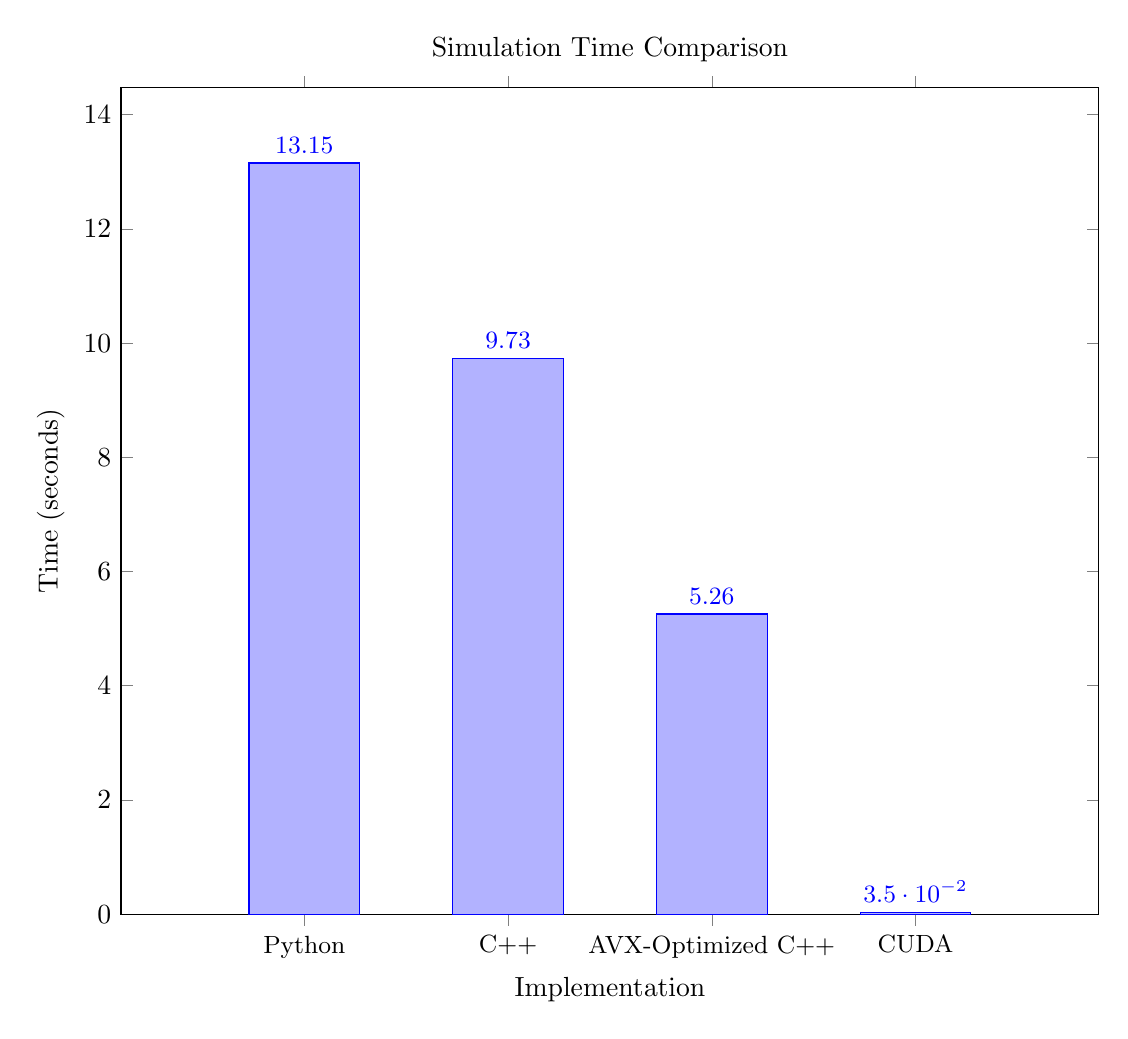
\begin{tikzpicture}
\begin{axis}[
    ybar,
    width=14cm,
    bar width=40pt,
    ymin=0,
    ylabel={Time (seconds)},
    symbolic x coords={Python, C++, AVX-Optimized C++, CUDA},
    xtick=data,
    nodes near coords,
    enlarge x limits=0.3,
    title={Simulation Time Comparison},
    xlabel={Implementation},
    nodes near coords style={font=\small},
    x tick label style={font=\small}, % slightly smaller labels
]
\addplot coordinates {(Python, 13.1546) (C++, 9.7335) (AVX-Optimized C++, 5.2558) (CUDA, 0.035)};
\end{axis}
\end{tikzpicture}
\end{figure}

\section*{Takeaways/Learnings}
\begin{enumerate}
    \item Normal vs Log-Normal Dstribution
    \item The \_ of geometric brownian motion (drift, volatility)
    \item NumPy functions for random number generation, summing along axis, etc
    \item Asian and barrier option payoff formulas
    \item Optimization methods like flat arrays and AVX
    \item Basic GPU paradigms and CUDA coding
\end{enumerate}

\end{document}